\section{Superblock distributions in deployed cryptocurrencies}

We measured the superblock distribution in the mainnet Bitcoin blockchain. Our
results are illustrated in Figure~\ref{fig.btc-superblocks}. As expected,
half the blockchain blocks are $1$-superblocks, $1/4$ of blocks are
$2$-superblocks and generally approximately $2^{-\mu}$ of the blockchain blocks
are $\mu$-superblocks. The horizontal axis denotes the block height, while the
vertical axis denotes the superblock density with respect to the variable
difficulty target of each block.

\begin{figure*}[h]
\begin{center}
  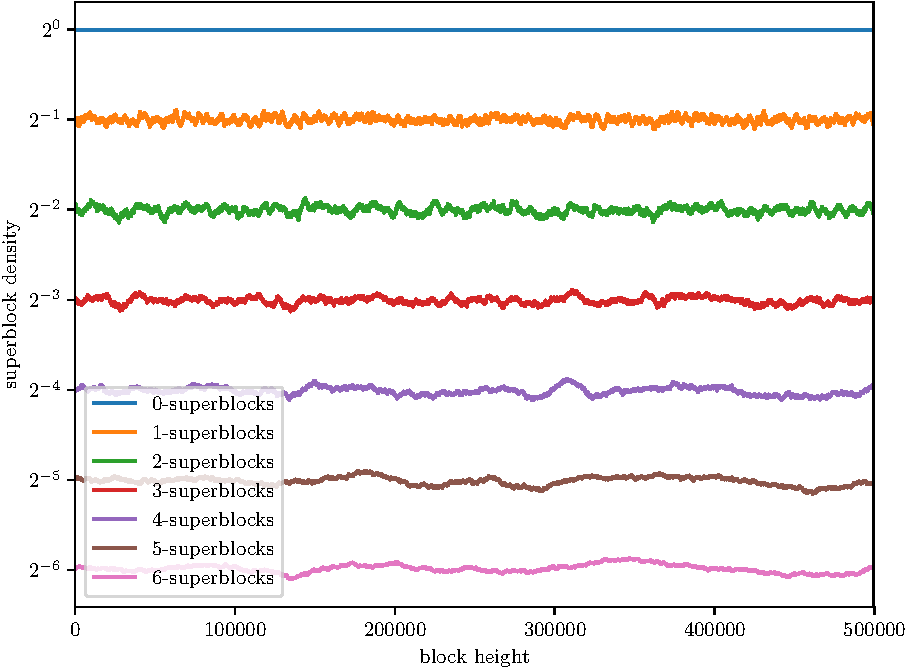
\includegraphics[width=0.95\textwidth]{figures/bitcoin-superblock-distribution.pdf}
  \caption{The distribution of block levels in Bitcoin. Superblocks are with
    respect to variable difficulty targets.}
  \label{fig.btc-superblocks}
  \end{center}
\end{figure*}
